
\begin{figure*}[h!]%
 \centering
 \subfloat[original]{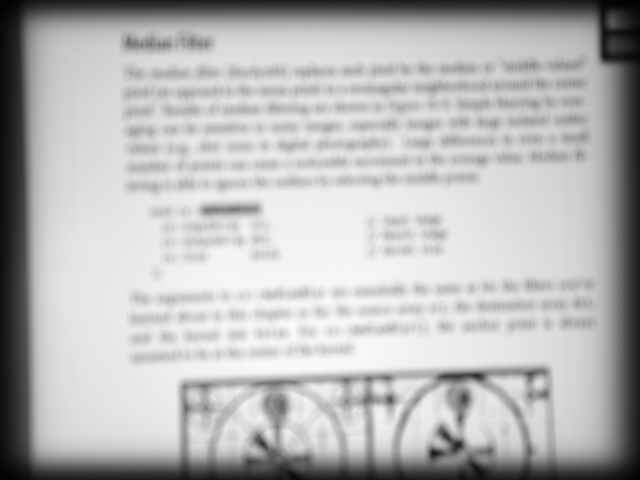
\includegraphics[width=\textwidth/2]{images/original.jpg}\label{fig:a}}\hspace*{3em}%
 \subfloat[background probability]{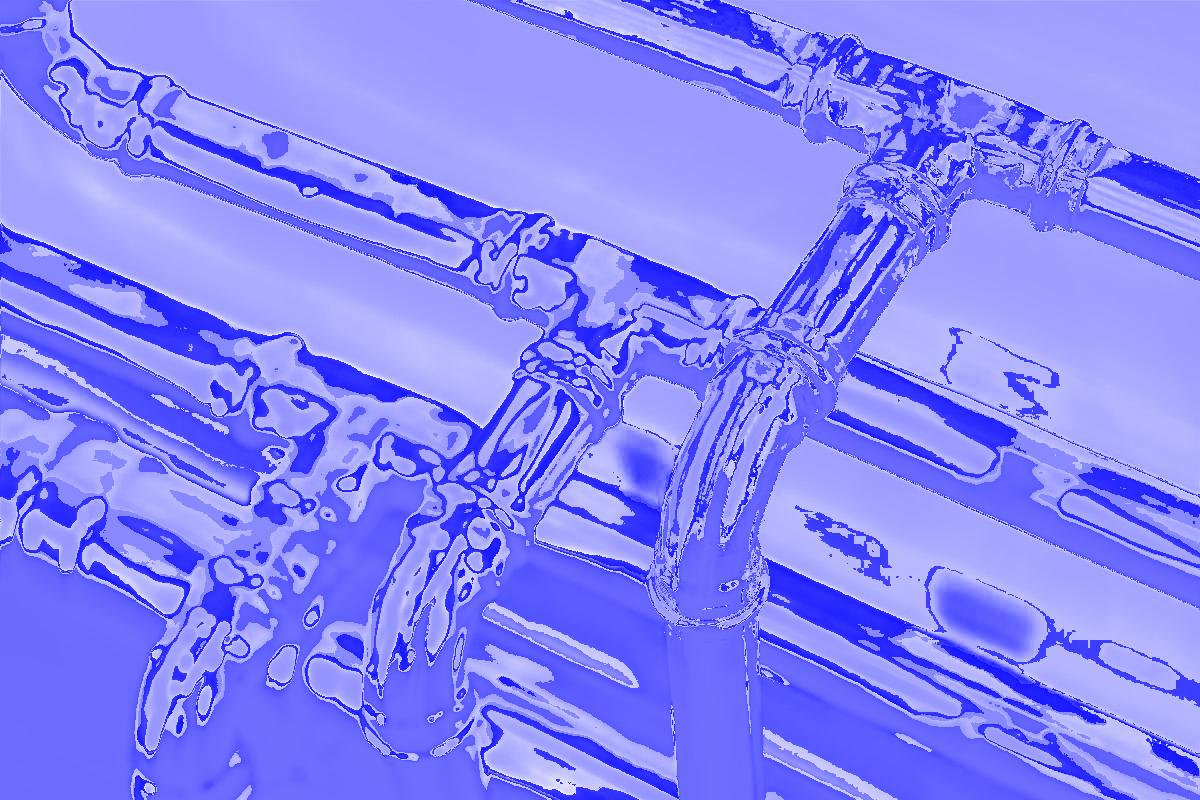
\includegraphics[width=\textwidth/2]{images/background-probability.jpg}\label{fig:b}}\\
 \subfloat[foreground probability]{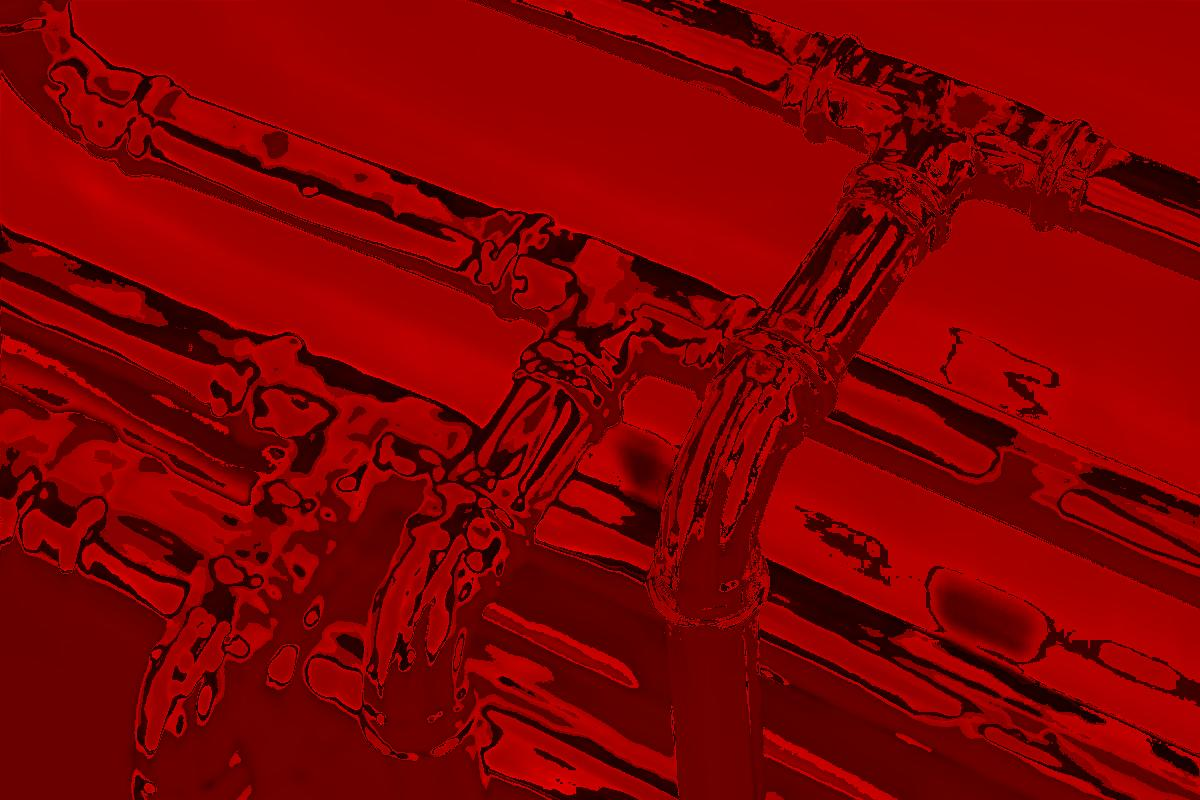
\includegraphics[width=\textwidth/2]{images/foreground-probability.jpg}\label{fig:c}}\hspace*{3em}%
 \subfloat[combined]{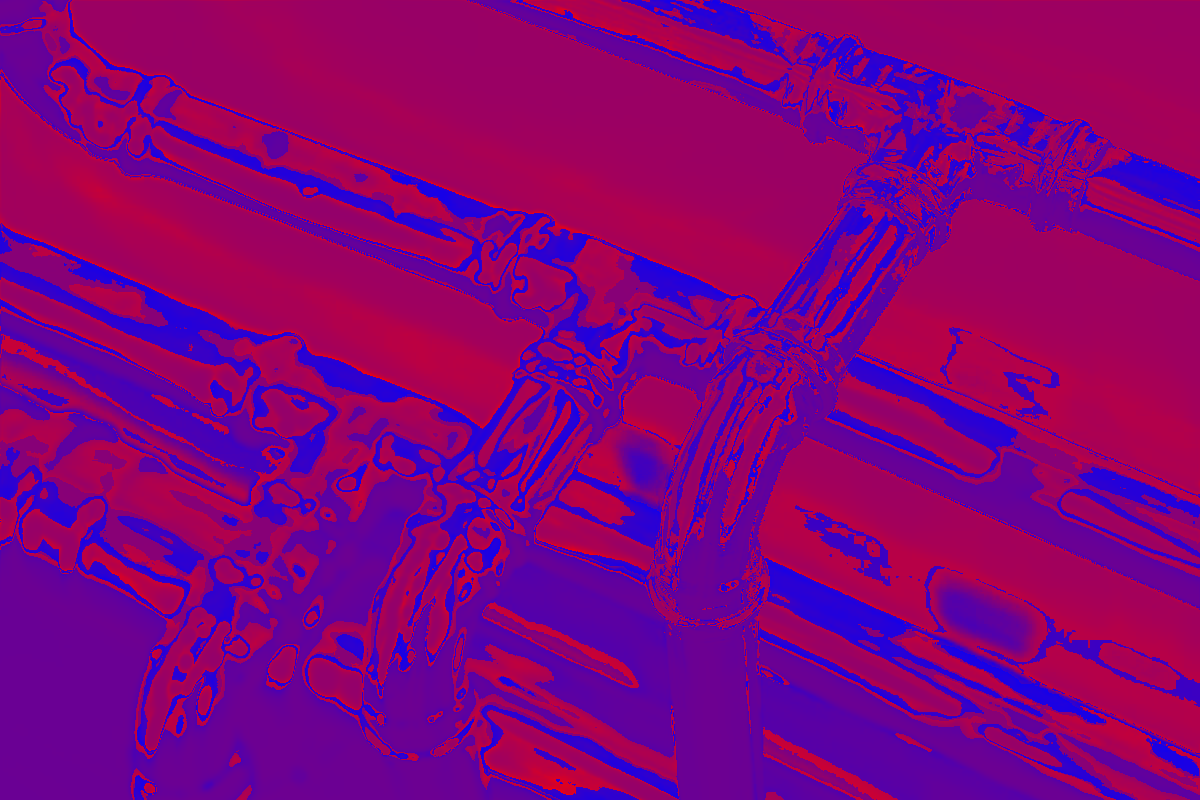
\includegraphics[width=\textwidth/2]{images/combined.png}\label{fig:d}}\\
 \caption{Background and Foreground Probability Scalars for Channel-Reduction}%
 \label{fig:all}%
(foreground probability is shown red-to-black, 
background is shown blue-to-white, and the 
two scales are merged in the combined graphic)
\end{figure*}


